\documentclass[conference]{IEEEtran}
% FORGE 2027 Data & Benchmarking track: IEEE conference template, 4 pages + 1 page of references,
% double-anonymous. The authors' own prototype is referred to as "G1".
\usepackage[T1]{fontenc}
\usepackage{graphicx}
\usepackage{booktabs}
\usepackage{amsmath}
\usepackage{url}
\usepackage[hidelinks]{hyperref}
\usepackage{xspace}
\newcommand{\rg}{\texttt{rg\,-w}\xspace}
\newcommand{\cbm}{codebase-memory\xspace}
\newcommand{\LARGEABSTRACT}{}\newcommand{\LARGECONTRIB}{}\newcommand{\LARGESECTION}{}\newcommand{\LARGETHREAT}{}

\begin{document}

\title{What Does ``N$\times$ Fewer Tokens'' Measure?\\Baselines, Sampling, and Output Form in\\Repository-Navigation Benchmarks}

\author{\IEEEauthorblockN{Anonymous Author(s)}\IEEEauthorblockA{Anonymized for review}}

\maketitle

\begin{abstract}
Code-graph tools for coding agents are promoted with large token-reduction ratios.
We ask how much such a ratio depends on how it is measured.
We contribute \textsc{NavBench}, a model-free benchmark whose labels never come from an evaluated tool:
seeded fixtures with known call sites, 17 public Python and TypeScript repositories with independently sampled targets, and calls observed while running the test suites.
We evaluate two Tree-sitter graph tools, ripgrep, and two language servers.
Re-applying our own prototype's earlier benchmark definition reproduces its headline: graph answers are 85$\times$ smaller than the whole files they replace.
The same answers are only 3.0$\times$ smaller than \rg output, and up to 2.2$\times$ \emph{larger} than compact language-server output.
Sampling targets from the prototype's own edges raises its answer rate from 44--54\% to 99--100\%; 32--42 points remain after adjusting for target composition.
For direct callers, the most complete graph tool used as many tokens as ripgrep on targets both answered completely (ratio 1.03, 95\% CI 0.94--1.13), but with far fewer wrong candidates (precision 0.98 vs.\ 0.35).
For depth-2 callers it needed 4.5$\times$ fewer tokens (0.22, 0.20--0.24).
\LARGEABSTRACT
We release the harness and data, and propose that efficiency claims report baseline, sampling frame, output form, completeness, and precision together.
\end{abstract}

\section{Introduction}
Coding agents spend much of their context budget locating code~\cite{bai_tokens}.
Graph-based navigation tools, exposed to the model as MCP tools, promise to answer structural questions such as ``who calls $X$?'' from a pre-built index~\cite{repograph,codexgraph,locagent,codebasememory}, and are often promoted with a token ratio.
A ratio has three hidden parameters that are not properties of the tool:
the \emph{baseline} (whole files, grep, or a language server),
the \emph{query sample} (often symbols the graph already connects),
and the \emph{output form} (names, locations, or source).
Our starting point was a research prototype by the authors, G1, whose own benchmark reported 85.8$\times$ fewer tokens than reading the referencing files, on graph-selected symbols; we evaluate G1 as one tool among others and report its failures.

We ask:
\textbf{Q1} How does the baseline change measured ratios?
\textbf{Q2} How does sampling targets independently of the graph change measured coverage?
\textbf{Q3} At matched completeness, with labels no tool produced, what do tools cost, for direct and for multi-hop callers?

\emph{Contributions:}
(1)~\textsc{NavBench}, an open harness with three independent label layers, automatic validity gates, and output-form control;
(2)~evidence that one set of graph outputs measures 0.45$\times$ to 139$\times$ depending on baseline and form;
(3)~a quantification of graph-conditioned sampling bias, adjusted for target composition;
(4)~matched-completeness costs showing no saving for direct callers but a 4.5$\times$ saving for depth-2 callers, with recall on runtime-observed calls\LARGECONTRIB.

\section{Benchmark Design}
\textbf{Tasks.}
T1 (primary): given a declaration, return its direct call sites (call expressions whose callee statically binds to it).
T2: given a call site, return the declaration.
T3 (added after freezing; fixtures only): callers up to depth 2.

\textbf{Layer A: seeded fixtures.}
A generator emits small executable Python and TypeScript repositories with one instance of each pattern:
direct calls; calls through an import alias, a module or namespace attribute, a re-export, a typed or \texttt{super} receiver; constructor and module-level calls; a same-named method on another class; a shadowing local; callbacks; string dispatch; decorators or arrow functions; and comment and string distractors.
Half use common, reused names.
A manifest lists every declaration and call edge; Python fixtures execute and TypeScript fixtures compile under \texttt{--strict}.
A gate requires the runtime-observed Python calls to equal the manifest; it caught three manifest omissions before any held-out data existed.
We use 4+4 calibration and 16+16 held-out fixtures (160 targets with explicit call sites), plus a second held-out split from fresh seeds.

\textbf{Layer B: natural repositories.}
9 Python and 8 TS/JS libraries, chosen by fixed criteria before any result.
Declarations are enumerated by tools sharing no code with any graph tool: Python \texttt{ast} and the TypeScript compiler API.
\emph{S-ind} (661 targets) is a stratified random sample of non-test declarations (strata: kind $\times$ language-server call fan-out; inclusion weights recorded).
\emph{S-cond} (331 targets) is drawn from declarations with $\ge$1 incoming G1 edge, the original benchmark's rule.
Layer B supports availability, size, and agreement, not accuracy.

\textbf{Layer C: runtime-observed calls.}
Each Python test suite runs under \texttt{sys.monitoring}; a call counts only when the callee's entry is confirmed.
Following dynamic-baseline evaluation of call graphs~\cite{totalrecall}, we report recall on observed calls; unobserved static results are not false positives.

\textbf{Tools.}
\rg with 0 and 3 context lines;
pyright 1.1.414 and the TypeScript 5.9.3 language service (\texttt{references}; native form: LSP \texttt{Location} JSON);
G1 \texttt{find\_references} and its original \texttt{lookup\_symbol}+\texttt{get\_dependencies} pair;
\cbm~\cite{codebasememory} at current main (\texttt{bf93f0b7}) and at v0.5.5, the release its paper evaluates.
v0.5.5 and v0.5.7 agree on every fixture query and differ on 5.8\% of natural queries, no more than v0.5.7 differs from its own re-run (5.3\%), so we report them as one row (``v0.5.x'').
Tools are queried through their own interfaces (MCP sessions for \cbm); a qualified name is sent only after a tool itself reports ambiguity.

\textbf{Scoring and statistics.}
Facts are mapped to call sites, enclosing callers, and files; an answer is \emph{complete} when caller recall is 1.
Tokens (cl100k; o200k changes \rg/graph ratios by $\le$0.06) are counted on native output, a common one-fact-per-line form, and a source-enriched form, with an automatic check that every form carries the same facts.
Estimates are repository-macro means with 95\% hierarchical-bootstrap intervals (repositories, then targets).
The primary contrast, the token ratio to \rg on targets both arms answer completely, and a 1.5$\times$ margin were frozen before held-out data.

\begin{figure*}[t]
\centering
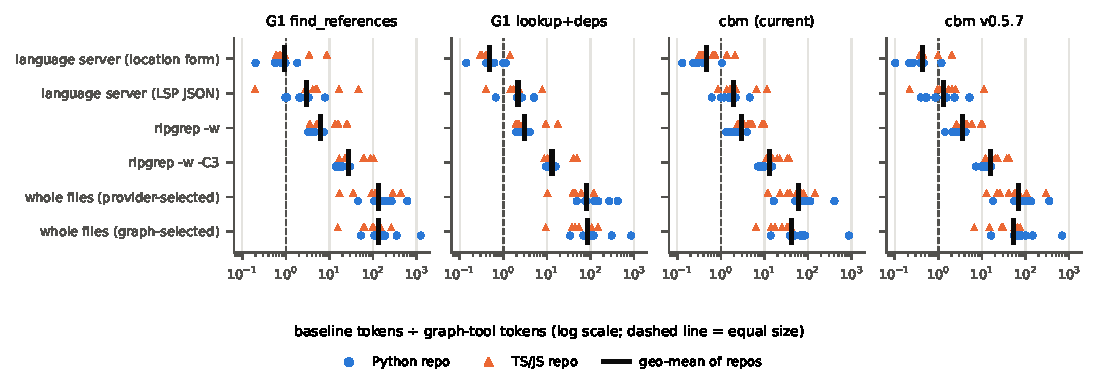
\includegraphics[width=\textwidth]{figs/fig1_q1_baselines.pdf}
\vspace{-1.6em}
\caption{Q1. Each baseline's payload divided by each graph tool's native output, for the same queries (S-ind, non-empty graph answers). Points: repository geometric means; bars: mean over repositories. Baseline and output form move the ratio by two orders of magnitude.}
\label{fig:q1}
\vspace{-0.8em}
\end{figure*}

\section{Results}
\subsection{Q1: the baseline determines the ratio}
Re-applying G1's original definition (graph-conditioned targets, whole files selected by the graph, \texttt{lookup}+\texttt{deps} output) to the public repositories gives 85.3$\times$ (95\% CI 57.2--126.9; 328 targets), matching the 85.8$\times$ originally reported.
This reproduces G1's own measurement only; it does not test \cbm's agent-level 10$\times$ result~\cite{codebasememory}, which measures a different workflow.
Against \rg the same outputs are 3.0$\times$ smaller (2.4--4.0), and against the language server printed one location per line they are larger (Table~\ref{tab:q1}, Fig.~\ref{fig:q1}).
On the 226 targets where every graph tool answered, the ordering is unchanged (\rg 2.5--4.7$\times$; LSP location form 0.45--0.86$\times$).
The \rg/graph ratio grows with the number of occurrences of the target's name (exploratory elasticity 0.77, CI 0.69--0.87): lexical search is costly mainly for common names.

\begin{table}[t]
\centering
\caption{Q1: baseline/graph payload ratio (repo-macro geometric mean, S-ind; each row over that tool's non-empty answers, n = targets).}
\label{tab:q1}
\setlength{\tabcolsep}{2.6pt}
\begin{tabular}{@{}lrrrrr@{}}
\toprule
Graph tool & n & whole files & \rg & LSP JSON & LSP loc.\\
\midrule
G1 find\_references & 358 & 139.3 & 6.01 & 3.10 & 0.88\\
G1 lookup+deps & 290 & 85.6 & 3.27 & 2.46 & 0.54\\
\cbm current & 395 & 48.0 & 2.92 & 1.92 & 0.45\\
\cbm v0.5.x & 413 & 60.8 & 3.54 & 1.46 & 0.46\\
\bottomrule
\end{tabular}
\vspace{-1em}
\end{table}

\subsection{Q2: graph-conditioned sampling overstates coverage}
S-cond also changes target composition: 9\% of its targets but 35\% of S-ind's have no call site according to the language server, and for those an empty answer is correct.
We therefore post-stratify S-cond to S-ind's distribution over repository $\times$ kind $\times$ fan-out bucket (0, 1--2, 3--9, $\ge$10).
The adjustment works as a control: the language server, on which S-cond is not conditioned, shows no adjusted difference (Table~\ref{tab:q2}).
For G1, the conditioning tool, 32--42 points of answer rate remain; its observed-call recall gap shrinks to +0.13 (CI reaching 0).
For \cbm the adjusted gap is 8--9 points: conditioning inflates mainly the coverage of the tool whose edges define the sample.
With the recorded inclusion weights, the S-ind answer rates fall further (\cbm current 60\%$\rightarrow$54\%).
G1 misses 14\% of independently sampled declarations; in five of eight TS/JS repositories its coverage is only 47--68\% (unindexed object-literal functions, collapsed same-named nested declarations).

\begin{table}[t]
\centering
\caption{Q2: S-cond $\rightarrow$ S-ind. Non-empty answers (\%), adjusted S-cond$-$S-ind difference [95\% CI], and caller recall on runtime-observed calls.}
\label{tab:q2}
\setlength{\tabcolsep}{3pt}
\begin{tabular}{@{}lccc@{}}
\toprule
Tool & non-empty \% & adjusted $\Delta$ (pts) & obs.-call recall\\
\midrule
G1 find\_references & 100 $\rightarrow$ 54 & +32 [21, 41] & 0.85 $\rightarrow$ 0.70\\
G1 lookup+deps & \phantom{0}99 $\rightarrow$ 44 & +42 [29, 53] & 0.81 $\rightarrow$ 0.63\\
\cbm current & \phantom{0}88 $\rightarrow$ 60 & \phantom{0}+9 [2, 17] & 0.79 $\rightarrow$ 0.66\\
\cbm v0.5.x & \phantom{0}84 $\rightarrow$ 62 & \phantom{0}+8 [0, 15] & 0.72 $\rightarrow$ 0.60\\
language server & \phantom{0}97 $\rightarrow$ 83 & \phantom{0}$-$1 [$-$5, 3] & 0.84 $\rightarrow$ 0.77\\
\rg & 100 $\rightarrow$ 100 & \phantom{$-$}0 & 0.97 $\rightarrow$ 0.95\\
\bottomrule
\end{tabular}
\vspace{-1em}
\end{table}

\subsection{Q3: cost at matched completeness}
\textbf{Direct callers (T1).}
Table~\ref{tab:q3} and Fig.~\ref{fig:q3} report the held-out fixtures.
The primary contrast is the geometric-mean token ratio to \rg over targets both arms answer completely; these subsets differ by arm and are conditioned on success.
A saving counts as meaningful only if the whole interval lies below $1/1.5\approx0.667$:
G1 \texttt{find\_references} 0.35 [0.33, 0.37] (n=64) and \cbm v0.5.x 0.58 [0.56, 0.62] (n=79) save, but are complete on only 40\% and 49\% of targets;
G1 \texttt{lookup}+\texttt{deps} 0.65 [0.62, 0.672] does not qualify;
\cbm current, the only graph tool as complete as the baselines, gives 1.03 [0.94, 1.13] (n=127): no evidence of a saving (not an equivalence test);
language-server JSON costs 1.75 [1.65, 1.85].
Without conditioning on completeness \cbm current's ratio is 1.01 [0.93, 1.09], and the fresh-seed split reproduces every contrast (\cbm current 1.02 [0.94, 1.12]).

Matched completeness is not matched quality: \cbm current returns almost no wrong callers (precision 0.98 vs.\ 0.35; F1 0.95 vs.\ 0.50).
The fixtures plant same-named methods, shadowing locals, and textual mentions, so they are deliberately hard for lexical search.
Form matters again: in the common one-fact-per-line form every graph tool needs only 0.24--0.28 of \rg's tokens on the same targets, so \cbm's native parity comes from its verbose tree output (160 vs.\ 19 tokens); graph lines name callers, whereas \rg lines list every occurrence.

\textbf{Depth-2 callers (T3, exploratory).}
Here the graph tool pays off: \cbm current is complete on 89\% of targets at 181 tokens, \rg on 80\% at 654, and on targets both complete it needs 0.22 [0.20, 0.24] of \rg's tokens (n=127) and 0.42 [0.38, 0.47] of the language server's.
The \rg strategy re-greps each caller and reads file outlines, a deliberately complete lexical baseline.

\textbf{Failures by pattern.}
\rg and pyright miss only calls through import aliases.
Of G1's 240 missed callers (\texttt{lookup}+\texttt{deps}), 96 resolve to a shadowing local, 32 are module-level calls, and 112 are unrecorded relations (re-exports, TS constructors, typed receivers).
Ambiguous names lower G1 \texttt{find\_references} recall from 0.73 to 0.53 but leave \cbm current unaffected.
In T2 every tool found every definition; only the language server returned exactly one.

\begin{figure}[t]
\centering
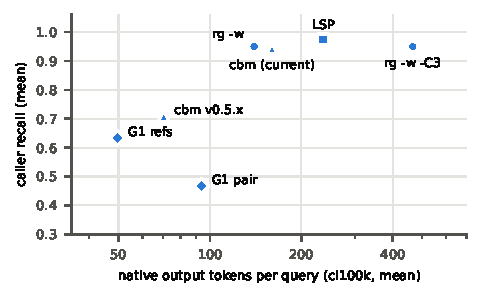
\includegraphics[width=\columnwidth]{figs/fig2_layerA_compact.pdf}
\vspace{-1.8em}
\caption{Q3, T1, held-out fixtures: native tokens vs.\ caller recall (repository means; G1 pair = lookup+deps). Small outputs coincide with low recall.}
\label{fig:q3}
\vspace{-1em}
\end{figure}

\begin{table}[t]
\centering
\caption{Q3: held-out fixtures (160 targets). Caller recall, precision, complete answers, and mean native tokens for direct callers (T1); complete answers and tokens for depth-2 callers (T3).}
\label{tab:q3}
\setlength{\tabcolsep}{2.4pt}
\begin{tabular}{@{}lrrrr|rr@{}}
\toprule
 & \multicolumn{4}{c|}{T1} & \multicolumn{2}{c}{T3}\\
Tool & rec. & prec. & compl.\% & tok. & compl.\% & tok.\\
\midrule
\rg & 0.95 & 0.35 & 80.0 & 140 & 80.0 & 654\\
language server & 0.97 & 0.64 & 90.0 & 236 & 90.0 & 402\\
G1 find\_references & 0.63 & 0.68 & 40.0 & 50 & 30.0 & 102\\
G1 lookup+deps & 0.47 & 1.00 & 40.0 & 94 & -- & --\\
\cbm current & 0.94 & 0.98 & 89.4 & 160 & 89.4 & 181\\
\cbm v0.5.x & 0.71 & 0.90 & 49.4 & 70 & -- & --\\
\bottomrule
\end{tabular}
\vspace{-1em}
\end{table}

\subsection{Layer C: recall on runtime-observed calls}
On 323 Python targets with observed calls (both samples, each target once), caller recall was
\rg 0.95 [0.92, 0.98], language server 0.79 [0.64, 0.90], G1 0.75 and 0.69, and \cbm 0.70 (current) and 0.64 (v0.5.x).
The gap is not explained by unindexed tests: on callers in library code the graph tools reach 0.63--0.76, against 0.94 for \rg and 0.86 for the language server.
Pyright's misses concentrate in repositories that ship \texttt{.pyi} stubs, to which it binds public-API calls.
The graph tools' recall is in the range reported for static Python call graphs~\cite{pycg}.

\LARGESECTION

\section{Recommendations}
\begin{itemize}
\item Report several baselines: one set of graph outputs measured 0.45$\times$ to 139$\times$.
\item Sample targets independently of the tool under test; sampling from G1's own edges added 32--42 points of answer rate after adjustment.
\item Count tokens in a common output form and state what it contains.
\item Report completeness and precision next to tokens, and separate single-hop from multi-hop queries: the same tool saved nothing on the first and 4.5$\times$ on the second.
\item Do not equate payload with agent cost~\cite{bai_tokens,weinberger}; agent-level studies~\cite{codebasememory,xu_lsp,codenib} measure something different.
\end{itemize}

\section{Threats to Validity}
\label{sec:threats}
\textbf{Construct.}
Payload tokens are not agent cost.
Labels encode one static semantics; caller-level scoring credits any location inside a true caller, but crediting only gold call sites changes recall by $\le$0.01.

\textbf{Internal.}
G1 is the authors' tool; every tool runs through its own interface under one frozen configuration, and G1's failures are reported in full.
Post-freeze changes, each released with before/after results:
a pyright readiness wait (layer-C recall 0.73$\rightarrow$0.79; Python targets were re-drawn with the same seed);
a scoring fix for the 76 targets drawn into both samples (S-ind numbers changed, conclusions did not);
\cbm v0.5.5;
T3, the fresh split, \LARGETHREAT and the robustness analyses (weights, common subset, strict credit, post-stratification).
\cbm v0.5.x answers for same-named declarations vary between runs (5\% of natural queries; current 0.4\%), and G1's answers vary when truncated at its output caps.

\textbf{External.}
Fixtures are cleaner than real code; repositories are a purposive selection in two languages; Layer C covers only exercised code; there is no human audit of natural-code accuracy.

\section{Related Work}
Code graphs improve repository-level tasks for agents~\cite{repograph,codexgraph,locagent}.
Agent-level studies report token savings under different setups: Codebase-Memory about 10$\times$ fewer tokens than a grep-and-read agent at lower answer quality (83\% vs.\ 92\%)~\cite{codebasememory}; CodeNib 50--87\% fewer tokens on SWE-bench issue queries under a quality-preserving margin~\cite{codenib}; Xu finds that language servers seldom save agent tokens and studies when they do~\cite{xu_lsp}.
Retrieval benchmarks score which files or snippets an agent should read~\cite{agentretrieval,corebench}; call-graph benchmarks score edges, with micro-benchmarks, LLMs, and dynamic baselines~\cite{pycg,swarm,dypybench,totalrecall}.
We instead score structural answers as context: their tokens at matched completeness, the sampling frame, and the output form, without a model.

\section{Data Availability}
Harness, fixture generator, pinned corpus commits, raw per-query outputs, traces, analyses, frozen protocol, and a one-command reproduction script: \url{https://anonymous.4open.science/r/XXXX} (anonymized).

\bibliographystyle{IEEEtran}
\begin{thebibliography}{99}
\bibitem{repograph} S.~Ouyang \emph{et~al.}, ``RepoGraph: Enhancing AI software engineering with repository-level code graph,'' in \emph{Proc. ICLR}, 2025.
\bibitem{codexgraph} X.~Liu \emph{et~al.}, ``CodexGraph: Bridging large language models and code repositories via code graph databases,'' in \emph{Proc. NAACL}, 2025.
\bibitem{locagent} Z.~Chen \emph{et~al.}, ``LocAgent: Graph-guided LLM agents for code localization,'' in \emph{Proc. ACL}, 2025.
\bibitem{codebasememory} M.~Vogel \emph{et~al.}, ``Codebase-Memory: Tree-sitter-based knowledge graphs for LLM code exploration via MCP,'' arXiv:2603.27277, 2026.
\bibitem{xu_lsp} P.~Xu, ``Does a language server save tokens for coding agents? A measurement methodology and preliminary study,'' arXiv:2608.13568, 2026.
\bibitem{codenib} Z.~Yu \emph{et~al.}, ``CodeNib: A multi-view data system for serving repository context to coding agents,'' arXiv:2607.25431, 2026.
\bibitem{agentretrieval} B.~Qin and Y.~Xie, ``Agent Retrieval Bench: Evaluating repository context retrieval for coding agents,'' arXiv:2607.24882, 2026.
\bibitem{corebench} F.~Zhang \emph{et~al.}, ``CORE-Bench: A comprehensive benchmark for code retrieval in the era of agentic coding,'' arXiv:2606.11864, 2026.
\bibitem{pycg} V.~Salis \emph{et~al.}, ``PyCG: Practical call graph generation in Python,'' in \emph{Proc. ICSE}, 2021.
\bibitem{swarm} R.~Venkatesh \emph{et~al.}, ``An empirical study of large language models for type and call graph analysis in Python and JavaScript,'' \emph{Empir. Softw. Eng.}, vol.~30, no.~6, 2025.
\bibitem{dypybench} I.~Bouzenia, B.~P.~Krishan, and M.~Pradel, ``DyPyBench: A benchmark of executable Python software,'' \emph{Proc. ACM Softw. Eng.}, vol.~1, no.~FSE, 2024.
\bibitem{totalrecall} D.~Helm \emph{et~al.}, ``Total recall? How good are static call graphs really?'' in \emph{Proc. ISSTA}, 2024.
\bibitem{bai_tokens} L.~Bai \emph{et~al.}, ``How do AI agents spend your money? Analyzing and predicting token consumption in agentic coding tasks,'' arXiv:2604.22750, 2026.
\bibitem{weinberger} S.~Weinberger and A.~Hozez, ``Token reduction is not cost reduction: An empirical study of end-to-end efficiency in API-based coding agents,'' arXiv:2607.12161, 2026.
\end{thebibliography}

\end{document}
